\documentclass{article}
\usepackage{amsmath}
\usepackage{xcolor}
\usepackage{amsthm}
\usepackage{graphicx}
\usepackage{hyperref}
\usepackage{datetime}
\usepackage{todonotes}

% inline comments
% you could use \listoftodos to print an overview
\newcommand{\inline}[1]{ {\color{blue}{#1}}\addcontentsline{tdo}{todo}{#1}}
\newcommand{\comment}[1]{{\color{blue}\noindent{#1}\\}\addcontentsline{tdo}{todo}{#1}}
% use this one to disable
%\newcommand{\inline}[1]{\ignorespaces}


\newdateformat{monthyeardate}{\monthname[\THEMONTH] \THEYEAR}

\newcommand{\newmarkedtheorem}[1]{%
  \newenvironment{#1}
    {\pushQED{\qed}\csname inner@#1\endcsname}
    {\popQED\csname endinner@#1\endcsname}%
  \newtheorem{inner@#1}%
}

\theoremstyle{definition}
%\newtheorem{eg}{Example}[section]
\newmarkedtheorem{eg}{Example}[section]
\newtheorem{observation}{Observation}[section]
\theoremstyle{plain}
\newtheorem{define}{Definition}[section]
\newtheorem{proposition}{Proposition}[section]
\newtheorem{theorem}{Theorem}[section]
\newtheorem{assump}{Assumption}[section]
\newtheorem{remark}{Remark}[section]


\title{Finite Buffers}
\author{Jeroen van Riel}
\date{\monthyeardate\today}

\begin{document}

\maketitle

\section{Model definition}

Up to this point, we have not taken into account the fact that lanes between
intersection have finite capacity. We need to incorporate this aspect in order
to develop a model that could be used for practical applications. Under high
traffic loads, lanes with finite buffer capacity can give rise to
\textit{blocking} of upstream intersections. Therefore, the traffic controller
needs to take into account these additional dynamics.

We start with a very simple extension of the single intersection scheduling
model that incorporates additional \textit{locations} on each lane. Instead of
only determining the arrival times of vehicles at intersections, the scheduler
has to determine the arrival and departure time of vehicles at every location.
We assume that it takes constant time $\Delta t$ for a vehicle to travel to the
next location.

For each lane $k \in \{1, \dots, K\}$, let $m_{k}$ denote the number of
locations, excluding the entrypoint. Let the locations of lane $k$ be identified
by increasing numbers $\mathcal{L}(k) = (1, \dots , m_{k})$, where the last one
corresponds to the final intersection. In the following variable definitions, we
will not explicitly mention the dependency on the lane to keep notation simple.
Let $y_{ij}$ denote the time at which vehicle $j$ departs from location
$i \in \{ 0, \dots, m_{k} \}$, then $y_{ij} + \Delta t$ is the arrival time of
vehicle $j$ at location $i+1$. To simplify notation, we define
$\bar{y}_{ij} = y_{i-1,j} + \Delta t$ to be the arrival time of vehicle $j$ at
location $i$. For every location $i$ and vehicle $j$, we require
\begin{align}
  \label{eq:constr1}
  \bar{y}_{ij} \leq y_{ij} .
\end{align}
For each pair of consecutive vehicles on the same lane $k$ with precedence
constraint $j \rightarrow l \in \mathcal{C}_{k}$, we have the inequalities
\begin{align}
  \label{eq:constr2}
  y_{ij} + p \leq \bar{y}_{il} ,
\end{align}
for every location $i$ along their route. Furthermore, we assume that for every
vehicle $j$, the initial departure time from the entrypoint of vehicle $j$ satisfies
\begin{align}
  \label{eq:release}
 r_{j} \leq y_{0j}
\end{align}
in order to model the \textit{arrival time} of the vehicle.

Finally, we need to model the safety constraints involving vehicles from
different lanes that cross the intersection. Let $j$ be some vehicle on lane
$k(j)$, then let let $y_{j}$ denote the departure time from the intersection, so
we have $y_{j} = y_{ij}$ with $i=m_{k(j)}$. Similarly, let $\bar{y}_{j}$ denote
the arrival time of $j$ at the intersection, so we have
$\bar{y}_{j} = y_{i-1,j} + \Delta t$ with $i = m_{k(j)}$. From
constraints~\eqref{eq:constr2}, we see that it makes sense to say that vehicle
$j$ occupies the intersection during the interval
\begin{align}
  [\bar{y}_{j}, y_{j} + p] .
\end{align}
Like in the single intersection scheduling problem, we require an additional
\textit{switch-over time} $s$ whenever the next vehicle to occupy the
intersection comes from a different lane. Therefore, we obtain a similar set of
constraints for the intersection. Like before, let
\begin{align}
  \mathcal{D} = \{ \{j, l\} : j \in F_{k_{1}}, l \in F_{k_{2}} , k_{1} \neq k_{2} \} ,
\end{align}
denote the set of \textit{conflict} pairs. The additional disjunctive
constraints are
\begin{align}
  \label{eq:3}
  y_{j} + p + s \leq \bar{y}_{l} \quad \text{ or } \quad y_{l} + p + s \leq \bar{y}_{j} ,
\end{align}
for all $j, l \in \mathcal{D}$.

Let $\mathcal{J}_{k}$ denote the set of all vehicles that approach the
intersection from lane $k$. Suppose we want to minimize total delay at the
intersection among all vehicles, then the extension of the single intersection
scheduling problem can be stated as
\begin{subequations}
\begin{align}
  \label{eq:finite-buffer-problem}
  \text{minimize } & \sum_{j} y_{j} \\
  \text{s.t. } & r_{j} \leq y_{0j} & \text{ for all } j, \\
               & \bar{y}_{ij} \leq y_{ij} & \text{ for all } j \in \mathcal{J}_{k} \text{ and } i \in \mathcal{L}_{k}, \\
               & y_{ij} + p \leq \bar{y}_{il} & \text{ for all } (j,l) \in \mathcal{C}_{k} \text{ and } i \in \mathcal{L}_{k}, \\
               & \text{either } \begin{cases} y_{j} + p + s \leq \bar{y}_{l} \\ y_{l} + p + s \leq \bar{y}_{j} \end{cases} & \text{ for all } \{j,l\} \in \mathcal{D} ,
\end{align}
\end{subequations}
where we let $k \in \{1, \dots, K\}$ implicitly to simplify notation.

\begin{define}
  \label{def:finite-buffer-problem}
  The problem defined be~\eqref{eq:finite-buffer-problem} is called the
  {\normalfont single intersection problem with finite buffers}.
\end{define}

\subsection{Alternative formulation}

We obtain a different perspective on the problem when we formulate it in terms of delay at locations instead of arrival and departure times.
For a vehicle $j$, we let
\begin{align*}
  d_{0j} = y_{0j} - r_{j}
\end{align*}
be the delay at its entrypoint.
For the remaining locations, we simply define
\begin{align*}
  d_{ij} = y_{ij} - \bar{y}_{ij} .
\end{align*}
It is not difficult to see that this is completely equivalent, based on the relationship
\begin{align}
  y_{ij} = r_{j} + i \cdot \Delta t + \sum_{n=0}^{i} d_{ij} .
\end{align}
When defining a reinforcement learning agent for generating trajectories, it
might be more sensible to generate $d$ instead of $y$.


\section{Solution}

We can solve~\eqref{eq:finite-buffer-problem} by formulating it as a MILP using
the big-M method and solve it using standard software. To illustrate the model,
let us consider a small example.

\begin{eg}
  \label{eg:finite-buffers}
  Let $\Delta t = 1$, $p = 1$ and $s = 1$ and consider two lanes with
  $m_{1} = m_{2} = 5$. Assume we have the following arriving vehicles
  \begin{align*}
    F_{1} = (1, 2) , F_{2} = (3, 4, 5)
  \end{align*}
  with arrival times
  \begin{align*}
    r = (0, 1, 2, 3, 5) .
  \end{align*}
  The optimal schedule has objective {\color{blue}todo} and is illustrated in
  Figure~\ref{fig:finite-buffer-example-schedule}.
\end{eg}

\begin{figure}
  \centering
  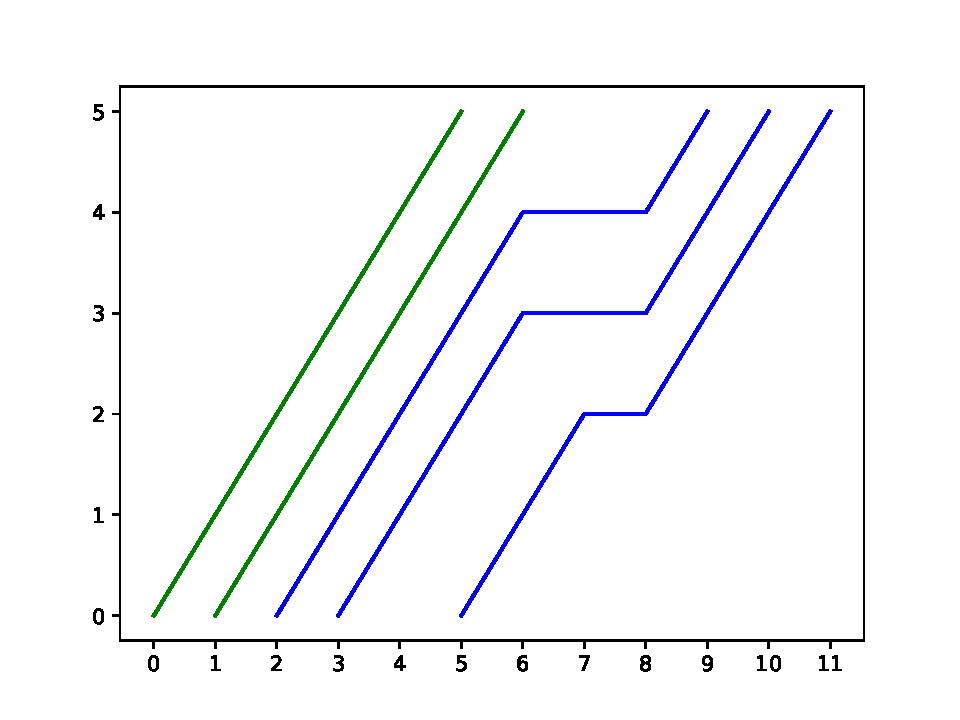
\includegraphics[width=0.9\textwidth]{figures/finite-buffer-schedule.pdf}
  \caption{Optimal schedule for Example~\ref{eg:finite-buffers}. The x-axis
    represents time and the location numbers are on the y-axis.}
  \label{fig:finite-buffer-example-schedule}
\end{figure}


\subsection{Reduction to single intersection scheduling problem}

{\color{gray} Recall the definition of a semi-active schedule. It turns out that
  there is always a schedule $y$ that is \textit{semi-active} at all locations
  except the intersection. <- This was my first thought, but it is not correct.}

We will show now that the problem above can be reduced to the single
intersection scheduling problem that we already discussed. It turns out that
there is always a schedule $y$ in which each vehicle always stays as close to
the next intersection as possible. -> find a definition for this! This means
that we can solve the single intersection problem to obtain $y_{j}$ and then
derive the rest of $y_{ij}$ from a simple recursive calculation.

\begin{proposition}
  The single intersection problem with finite buffers has an optimal schedule
  that is [insert definition here].
\end{proposition}
\begin{proof}
  Suppose $y$ is some optimal schedule. We show how to derive from this a
  schedule $y'$ that is semi-active at all locations other than the intersection
  without increasing the objective.

  We set $y'_{j} = y_{j}$ for all $j$, so the objective does not change. Now for
  each lane $k$, we derive the remaining $y_{ij}$ for the vehicles
  \begin{align*}
    j_{1} \rightarrow j_{2} \rightarrow \dots \rightarrow j_{n_{k}} .
  \end{align*}
  on this lane. Let $\mathcal{C}_{k}$ denote the set of all precedence
  constraints between vehicles of this lane.

  Since the intersection is the last location, a vehicle can always continue
  immediately after reaching it. Therefore, we do not have to wait at the
  intersection, so we set $y'_{m(k),j} = \bar{y}'_{m(k),j}$ for all $j_{1},\dots, j_{n_{k}}$, so
  that we have $y'_{m(k)-1,j} = y'_{m(k),j} - \Delta t = y_{j} - \Delta t$.

  For the first vehicle $j_1$, we can simply set
  \begin{align*}
    y'_{ij_{1}} = y'_{i+1, j_{1}} - \Delta t ,
  \end{align*}
  for $i \in \{1, \dots, m(k) -1 \}$.
  For every pair of consecutive vehicles
  $j \rightarrow l \in \mathcal{C}_{k}$, we set
  \begin{align*}
    y'_{il} = \min \{ y'_{i+1, l} - \Delta t, y'_{i+1, j} + p - \Delta t  \},
  \end{align*}
  for $i \in \{1, \dots, m(k) -1 \}$

  From these recursive equations, all values of $y'$ can be determined. It is
  not difficult to see that $y'_{il}$ cannot be made smaller without increasing
  another entry of $y'$, because it needs to satisfy
  $y'_{il} + \Delta t = \bar{y}'_{i+1,l} \leq y'_{i+1,l}$ and
  $y'_{il} + p \leq \bar{y}_{il}$.
\end{proof}



\section{Extending to network}

It is not a surprise that we can reduce the problem back to the variant with
infinite buffer space, because we essentially still have infinite buffer space
at the entrypoints. The only difference is that the movement is now somewhat
more explicitly modelled. As we move on to consider more than one intersections,
we will see that the model is really different.

{\color{gray} For every lane $(x_{0}, x_{1})$, let $m(x_{0}, x_{1})$ denote the
  number of locations between both endpoints. Consider vehicle $j$ with route
  $R_{j}$. Let $y_{ij}$ denote the time at which vehicle $j$ departs from
  location $i = R_{j}(k)$ for some $k$, then $y_{ij} + \Delta t$ is the arrival
  time of vehicle $j$ at location $R_{j}(k+1)$. To simplify notation, we define
\begin{align}
  \bar{y}_{ij} = y_{R_{j}(k-1),j} + \Delta t
\end{align}
to be the arrival time of vehicle $j$ at location $i = R_{j}(k)$. For every
location $i$ and vehicle $j$, we require
\begin{align}
  \bar{y}_{ij} \leq y_{ij} .
\end{align}
For each pair of consecutive vehicles on the same lane
with precedence constraint $j \rightarrow l$, we have the inequalities
\begin{align}
  y_{ij} + p \leq \bar{y}_{il} ,
\end{align}
for every location $i$ along the shared parts of their routes. Furthermore, we
assume that for every vehicle $j$, the initial departure time from the first
location $i_{0} = R_{j}(0)$ on the route of vehicle $j$ satisfies
\begin{align}
  \label{eq:release}
  y_{i_{0},j} \geq r_{i_{0},j}
\end{align}
in order to model the \textit{release date}.
}


\section{Second order constraints}

Our initial formulation is rather unrealistic, because it allows, in some sense,
infinite acceleration. In order to model bounded acceleration, we will consider
additional constraints on the difference between delay at consecutive locations.
More specifically, we require
\begin{align*}
  d_{i-1,j} - d_{ij} \leq a ,
\end{align*}
for all vehicles $j$ and locations $i \in \mathcal{L}(k) \setminus \{ 1 \}$.
In terms of $y$, we obtain the usual finite differences
\begin{align*}
  y_{ij} - 2 y_{i-1,j} + y_{i-2,j} \leq a .
\end{align*}
often seen in numerical analysis.


% \bibliography{references}
% \bibliographystyle{ieeetr}

\end{document}
